\documentclass[oneside,a4paper,10pt,parskip=full,toc=listof]{scrreprt}
\setcounter{secnumdepth}{3}
\setcounter{tocdepth}{3}

%\usepackage{tuwien} %Fürs Titelblatt

%\usepackage{ucs} %für Unicode Support
\usepackage[utf8]{inputenc} %für Unicode Support des Editors
\usepackage[ngerman]{babel} %Silbentrennung
\RequirePackage[ngerman=ngerman-x-latest]{hyphsubst} %Zusammengesetzte Wörter werden besser getrennt (zB Glasplatte)
\usepackage[T1]{fontenc} %Vektorschrift verwenden
\usepackage{graphicx} %einbinden von Bitmaps und PDFs


\usepackage{bibgerm} %Literaturverzeichnis

\usepackage[fleqn]{amsmath} %für zB \dfrac
\usepackage{amssymb}
\usepackage{units} %Einheiten darstellen
\usepackage{nicefrac} %Brüche von Einheiten darstellen
\newcommand{\gap}{\ldots \ldots \ldots} %Punkte für Lückentext
\newcommand{\ef}[1]{_{ef\!f,#1}} 
\newcommand{\eff}{_{ef\!f}}

% automatische Anpassung der Seitenränder
\usepackage[inner=3cm, outer=2cm]{geometry}

%Kopf- und Fußzeilen anpassen
\usepackage{scrpage2} 
\pagestyle{scrheadings}
\automark{chapter}
% ohne Kapitelnummern
\renewcommand{\chaptermark}[1]{\markleft{#1}}
% \renewcommand{\sectionmark}[1]{\markright{#1}}
% löscht vordefinierte Kopf und Fußzeilen
\clearscrheadfoot
\ohead{\leftmark} 
% \ohead{\rightmark}
\setheadsepline{0.4pt}
\ifoot{Michael Fuchs, 9725501} 
\cfoot{}
\ofoot{\pagemark} 
\setfootsepline{0.4pt}

%Formatierung der Links im Dokument (zB Inhaltsverz)
\usepackage[colorlinks=true,
        linkcolor=black,
        citecolor=black,
        filecolor=black,
        urlcolor=black,
        bookmarks=true,
        bookmarksopen=true,
        bookmarksopenlevel=3,
        plainpages=false,
        pdfpagelabels=true]{hyperref}


%zum Einbinden von Grafiken aus Inkscape via PSTricks
% strichlierte Linien passen tw. nicht, daher jetzt PDF als Grafikformat
% \usepackage{pst-all}
% \usepackage{pst-pdf}

%ScaleIfNeeded für Grafiken, die breiter als Seitenbreite sind.
\makeatletter
\def\ScaleIfNeeded{%
\ifdim\Gin@nat@width>\linewidth
\linewidth
\else
\Gin@nat@width
\fi
}
\makeatother

%zum Erstellen von Plots
% \usepackage{tikz}\usepackage{tikz}
\usepackage{pgfplots}
\usepgfplotslibrary{units}
\pgfplotscreateplotcyclelist{color list}{%
red,blue,black,brown,teal,orange,violet,cyan,green!70!black,magenta,gray,yellow}
\pgfplotscreateplotcyclelist{mymarks}{%
      red,mark=*\\%
      blue,mark=square*\\%
      black,mark=otimes*\\%
      brown,mark=star\\%
      teal,mark=diamond*\\%
      red,densely dashed,every mark/.append style={solid,fill=red!80!black},mark=*\\%
      brown!60!black,densely dashed,every mark/.append style={
      solid,fill=brown!80!black},mark=square*\\%
      black,densely dashed,every mark/.append style={solid,fill=gray},mark=otimes*\\%
      blue,densely dashed,mark=star,every mark/.append style=solid\\%
      red,densely dashed,every mark/.append style={solid,fill=red!80!black},mark=diamond*\\%
}
\pgfplotsset{
      compat=1.3,
      tick label style={font=\small},
      label style={font=\small},
      legend style={font=\scriptsize},
      cycle list name=color list
}

% TxODO PGF Farben der Graphen anpassen
% TxODO PGF Farben der Marks anpassen

%Formatierung von Tabellen
\usepackage{dcolumn}
\usepackage{booktabs}

%check ich noch nicht ganz. Spalten sollen nach Dez.punkt ausgerichtet werden:
\makeatletter
\newcolumntype{d}[1]{%
>{\DC@{,}{,}{#1}}l<{\DC@end}%
}
\makeatother

%multicol für einzelne Spalte (Trick)
\newcommand{\tk}[1]{\multicolumn{1}{c}{#1}}

% fuer Stichwortverzeichnis
\usepackage{makeidx}
% Stichwortverzeichnis erstellen
\makeindex

% todo-notes im Text einfügen
% \setlength{\marginparwidth}{2cm}
% \usepackage[textsize=tiny,shadow]{todonotes}

\def\daVersion{0.01} %laufende Versionsnummer



\begin{document}

    \title{Experimentelle und theoretische Untersuchungen zu Holz-Glas-Verbundplatten}
    \author{Michael Fuchs}
    \matrnr{9725501}
    \addreins{Braunhirschengasse 5/13}
    \addrzwei{1150 Wien}
    \institut{Architekturwissenschaften, Tragwerksplanung und Ingenieurholzbau}
    \institutsnr{E259/2}
    \betreuer{o.\,Univ.\,Prof.\,DDI\,Wolfgang Winter}
    \studienort{Wien}
    \damonat{März} % Abgabemonat
    \datag{11} % Abgabetag
    \dajahr{2012}  % Abgabejahr

\titelseite
% \clearemptydoublepage
% \copyrightseite

%Seitenzahlen mit römische Ziffern bis Inhaltsverzeichnis
\setcounter{page}{1}
\pagenumbering{Roman}

\erklaerung


%Inhaltsverzeichnis
\tableofcontents


% Seitenzahlen mit arabische Ziffern (sh. symbole.tex)
% \setcounter{page}{1}
% \pagenumbering{arabic}

%Kapitel Symbole

\chapter{Einführung}
\section{Einleitung, Ziele und Vorgehensweise}
 

Die vorliegende Diplomarbeit entstand im Rahmen  der Forschungstätigkeit am Institut für Tragwerkplanung und Ingenieurholzbau. Sie schließt an die Arbeiten von  Kirchmayer [1] \cite{1} und  Schernberger [2] an. Im Rahmen des Forschungsprojektes "`Weitgespannte Flachdeckensysteme in Holzspanbeton – Verbundweise"'  sind ihre Arbeiten entstanden. Die Ausarbeitung von Schernberger befasst sich mit der allgemeinen Anwendung und den Einsatzgebieten des Holzleichtbetons. Kirchmayer hat anhand von Versuchsreihen das Tragverhalten- und Verformungsverhalten verschiedener Aufbauten und Verbindungsmittel untersucht.  Durch diese Versuche und Analysen ist der dargestellte Sandwichaufbau \ref{sandwich} entstanden. 



\begin{figure}[h!]
\begin{center}
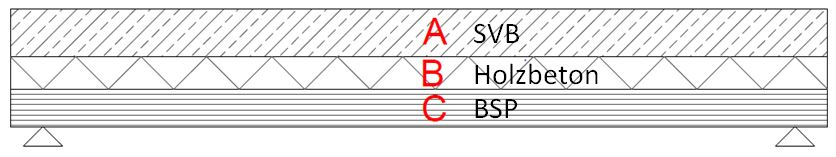
\includegraphics[scale=0.7]{Einleitung/sandwichaufbau.JPG}
\caption{Sandwichaufbau}
\label{sandwich}
\end{center}
\end{figure}

\subparagraph{Ziele und Vorgehensweise:}

Das erste übergeordnete Ziel dieser Arbeit ist die Entwicklung eines Sandwichaufbaus aus Brettsperrschichtholz (BSP), Holzleichtbeton und selbeverdichtendem Beton\,(SVB). Der SVB nimmt in dem Aufbau die Druckschicht ein, das BSP die Zugschicht und der Holzleichtbeton die Mittelschicht. Die Verbindung der unterschiedlichen Werkstoffe wird durch die Anwendung von Schrauben und einem Kleber gewährleistet. Das zweite Ziel dieser Arbeit ist die Nachrechnung der Versuchsergebnisse mit den „$\gamma$ -Verfahren“ und dem Finite Elemente Programm „Sofistik“. Es sollen die Grundlagen zur Bemessung des Sandwichaufbaus entwickelt werden. 
Zusätzlich ist eine ökonomische Betrachtung des Sandwichaufbaus zu erstellen und einen Vergleich mit den gängigen Deckensystemen zu erarbeiten.\newline Die genannten Ziele sollen mit Hilfe von den experimentellen Großbauteilversuchen erreicht werden. Dabei wird ausschließlich das Kurzzeitverhalten des Sandwichaufbaus untersucht. Die Kurzzeitdurchbiegung wurde mit l/400 begrenzt, um Reserven für Langzeitverformungen aufzubringen.




\newpage{}
Im Nachfolgenden Ablaufdiagramm ist die Vorgehensweise bei der Erstellung der Arbeit ersichtlich.

\begin{figure}[h]
\begin{center}
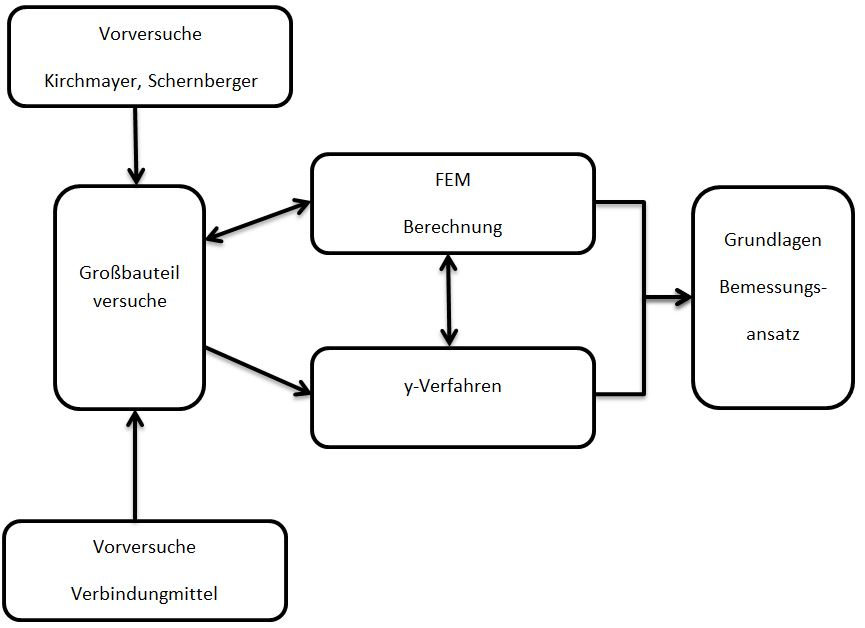
\includegraphics[scale=0.7]{Einleitung/ablauforganigramm.JPG}
\caption{Ablauforganigramm der Diplomarbeit}
\end{center}
\end{figure}




\section{Zusammenfassung der Kapitel}

\begin{enumerate}
\item Zusammenfassung von Vorarbeit 
\item Ermittlung der mechanischen Eigenschaften der Verbindungsmittel
\item Versuchaufbau und Durchführung
\item Beschreibung und Auswertung der Großbauteilversuche
\item Beschreibung der Berechnungsverfahren
\item Vergleich Berechnung Versuche und Berechnungen
\item wirtschaftliche Untersuchungen

\end{enumerate}



%Verzeichnisse
\newpage
% \addcontentsline{toc}{chapter}{Verzeichnisse}

\listoffigures
% \addcontentsline{toc}{section}{Abbildungsverzeichnis}

\newpage
\listoftables
% \addcontentsline{toc}{section}{Tabellenverzeichnis}

\newpage
% Index soll Stichwortverzeichnis heissen
\renewcommand{\indexname}{Stichwortverzeichnis}
% Stichwortverzeichnis endgueltig anzeigen
\printindex
% Stichwortverzeichnis soll im Inhaltsverzeichnis auftauchen


% Literaturverzeichnis
\newpage
\nocite{*}

\bibliographystyle{alphadin}
\bibliography{HGV}
% \listoftodos
\end{document}
